\chapter{Conclusions and Future Work}

\section{Conclusions}

Minimally invasive surgery robotics is a fascinating area of robotics research that has a huge impact in improving surgical operations, but is also very demanding and complex in implementation. Due to the nature of the tasks 
the surgical robots must execute, that is to operate on patients, the implemented solutions must have very strict requirements in accuracy and quality assurance. The critical requirements that were studied in this thesis are 
discussed in more detail below.\\

\textbf{Positional accuracy}: The trajectories that the robot executes (especially the pivot trajectories inside the surgical site) must be executed with micrometer accuracy. This positional accuracy is required for both the end-
effector as well as for the tip of the surgical tool. It is important to note, that due to the fulcrum effect a small error in the end-effector can cause a bigger error in the position of the tool tip and vice-versa. Errors 
in a magnitude that is bigger than the magnitude of micrometers can cause serious surgical side-effects and can also be fatal. The experiments of this thesis were conducted with the requirement of bounding the position error 
of the end-effector to $\pm 5μm$, but smaller values are recommended (if possible). The positional accuracy in trajectories outside of the patient body, like for example approaching the table of the surgical tools to execute a 
pick-and-place pipeline, is not as strict and was increased to $0.5mm$.\\

\textbf{Orientation accuracy}: Similar to the positional accuracy, orientation accuracy is also very crucial for both the end-effector and the tip of the surgical tool, and it also sometimes affects the deviation error from the 
fulcrum point. Orientation errors can also have negative side-effects in the surgical operation and small errors in the end-effector can cause bigger errors in the tool tip and vice-versa. The experiments of this thesis were 
conducted with the requirement of bounding the orientation error of the end-effector to $\pm 5\cdot 10^{-6}$degrees. The orientation accuracy in trajectories outside of the patient body, is not as strict and was increased to 
$\pm 5\cdot 10^{-4}$degrees.\\

\textbf{Time optimization}: Time optimal trajectories in the context of this thesis means to find the paths, avoiding collisions and respecting the constraints as well as calculating the trajectories in the shortest amount of time as 
possible. This is very important, so that the robot can be responsive in real-time to the surgeon’s commands and to be able to quickly and safely execute a given task. In all experiments a maximum of 5 seconds was specified 
for each path planning request. Although this time duration is significantly big, many experiment path planning requests were completed in less than a second 
(see measurements from \ref{section:robot-planner1}, \ref{section:robot-planner2}, \ref{section:robot-planner3b}).\\

\textbf{RCM constraint}: The Remote Center of Motion constraint is the one of the most important constraints in minimally invasive surgeries (see also section \ref{rcm-subsubsection}). To satisfy this constraint, all trajectories were designed using 
spherical coordinates with respect to the fulcrum reference frame. To make sure that the surgical tool satisfies this constraint a RCM error metric was used to measure the distance of the line of the long axis of the tool 
from the fulcrum point. This error was mostly measured for the insertion, retraction and line segment trajectories with very satisfactory results with the errors being in the magnitude of micrometers 
(see figure \ref{robot-planner3b-line-seg-rcm-errors}). It is important to keep this error at a minimum to avoid exerting pressure to the patient’s abdominal wall.\\

\textbf{Interpolation accuracy}: This requirement states that the number of interpolated waypoints of a path/trajectory should be enough such that the geometry of the path is not significantly distorted, for example a circular 
trajectory designed in the taskspace should have enough sample points so that the approximated polygon will be close to the desired circle. Choosing 4 sample points for example for a circular trajectory would reduce the 
circle to a square trajectory. In this thesis the interpolation is done at two stages, the first stage is the one already mentioned and the second is a lower level interpolation made by MoveIt path planner when executing 
cartesian line paths. For this second interpolation, a step distance is defined such that the actual executed path is as close to the line as possible (see figure \ref{interpolation-accuracy}). In the experiments, the 
geometric interpolation was made using 20 or 50 sample points and the second interpolation was made using a step size of 1mm. For both parameters, a higher choice is recommended for more precise movements but with an extra 
cost of heavier computational requirements.\\

\textbf{Collision avoidance}: This requirement is common in most robotic applications and it means that the path planning algorithms must take into consideration the environment obstacles and execute trajectories around them without 
colliding with them. In most cases this requirement was automatically satisfied from the MoveIt framework, where it was specified that each kinematics solution should be collision-aware. The second case that was not handled 
by MoveIt and was separately handled in the experiments was the elbow-up constraint. This constraint (see also \ref{section-elbow-up-constraints}) was purposefully imposed so that the robot arm’s elbow would not collide with 
the mounting dock (the object with the trocars that simulates the patient) when executing pivot motions.\\

\textbf{Suitable path planning algorithms}: The MoveIt motion planning framework for ROS provides a wide range of path planning algorithms to choose from. The requirements for choosing a path planning algorithm were to find a 
collision-aware solution in the shortest time possible, respecting all constraints, without any replanning (if possible) and to provide under the same conditions the same results. In the first experiment the two algorithms 
that were benchmarked were the RRTConnect and the RRT* algorithms and all other experiments were conducted using the RRTConnect algorithm, which provided satisfactory time results and is also the default path planning 
algorithm in MoveIt.\\

\textbf{Repeatability} \& deterministic results: When studying robotic applications one other metric that one should study other than the accuracy, is the robot’s repeatability. The repeatability measures how “close” the measurements 
are with each other or in terms of statistics, what is the standard deviation of the measurements. A good repeatability is achieved when the standard deviation is as small as possible. In this thesis, all measurements were 
generated from running each experiment at least 10 times, in order to calculate the average and the standard deviation. Deterministic results in the measurements, in the context of this thesis, means that the measurements are 
not random and are predicted to be close to the average measurement and within a range of two or three standard deviations.\\

\textbf{Good environment layout and robot base position}: When choosing how to position the robot in the operating room and how to set up the objects’ layout it is very important to take into consideration the robot’s available 
workspace. The surgical tools’ positions that the robot must approach, and the surgical site, where the robot must operate at, must be fully inside the robot's workspace and be well reachable, which means that the robot must 
be able to reach a desired position with ease and flexibility. In the first 2 experiments, there was used a layout that made it difficult for the robot to reach all surgical tools and trocar points, so in the rest of the 
experiments a different layout was used, where the robot was much closer to the tools and the surgical site and could execute the pivot trajectories with more flexibility.\\

\textbf{Good reachability of trajectories}: Similar to the good layout discussed above, the trajectories, especially those of the pivot motions, must be designed in such a way so that the robot can fully follow them with ease and 
flexibility. The “flexibility” term means, to operate at points away from singularity points, away from the workspace boundary and without “weird” poses that make the robot to “self-fold” or even worse to self-collide.\\

\textbf{Singularity avoidance}: This requirement is also common in all robotic applications but is even more important in surgical robotics. When in a singularity point, the robot loses one or more kinematic degrees of freedom and 
cannot move or moving at a singularity point would require huge effort from the joints. Both cases could result in surgical side-effects, as well as cause problems to the robot and should always be avoided. Singularity points 
are avoided from the MoveIt framework when calculating the paths, and are also avoided in the lower-level controllers of the robot’s real hardware. Singularity point approaching was also tracked using the robot’s Jacobian and 
the manipulability index (see figure \ref{robot-planner1-manipulability-plot}).\\

\textbf{Jump threshold}: This is an important parameter when executing trajectories with real robot hardware and reduces the large unpredictable motions of redundant joints that could be a safety issue (in this case both for the 
patient and the operating staff). These undesirable motions can occur when the arm approaches singularities and needs to reorient the arm in order to continue following the trajectory. In simulation experiments this parameter 
was disabled to better study the path planning in all possible cases, but this is highly not recommended when operating real robot hardware. The jump threshold parameter can be more relaxed in pick and place pipelines because 
there the robot has more flexibility to move, but it must be more restricted when executing pivot motions.\\

The conclusions above were drawn given some \textbf{assumptions} that were taken into consideration to simplify, without loss of generality, some experiments. The assumptions were the following:
\begin{itemize}
\item The \textbf{fulcrum position and orientation} were assumed known and constant. All trajectories from the experiments were calculated using constant fulcrum reference frames, which according to the bibliography in more 
realistic scenarios is not the case, and the pose of a fulcrum point is usually estimated.
\item The surgical tool appears fixed on the end-effector of the robot. In this thesis a higher level overview of \textbf{surgical tool grasping} was studied in order to better study the pivot trajectories separately without 
the being affected by grasping forces and fulcrum-tool torques.
\item The simulation environment features were assumed known and constant, which means that the pose of the surgical tools and the trocar were assumed known and their values were not extracted from the \textbf{Computer Vision 
node} that calculated these poses using a stereoscopic camera.
\end{itemize}

The goal of this thesis was to study in an \textbf{end-to-end approach}, all the stages involved in the recognition, control and manipulation of laparoscopic tools, but \textbf{more emphasis was given to the pivot 
trajectories and the RCM constrained motion planning}. Since this approach is very complex and involves many different algorithms, mathematics, techniques and technologies, it was very useful that each stage was studied 
separately and isolated to make sure that each stage performs well on its own (unit testing), so that later all stages can be integrated and studied together (integration testing). A higher level end-to-end pipeline that can 
be used for integration testing is proposed in the state machine of \ref{section:robot-planner7}. \\




\section{Future Work}

\textbf{Simulation and interaction with deformable bodies} \\

\begin{center}
\begin{figure}[!htb]
\centering
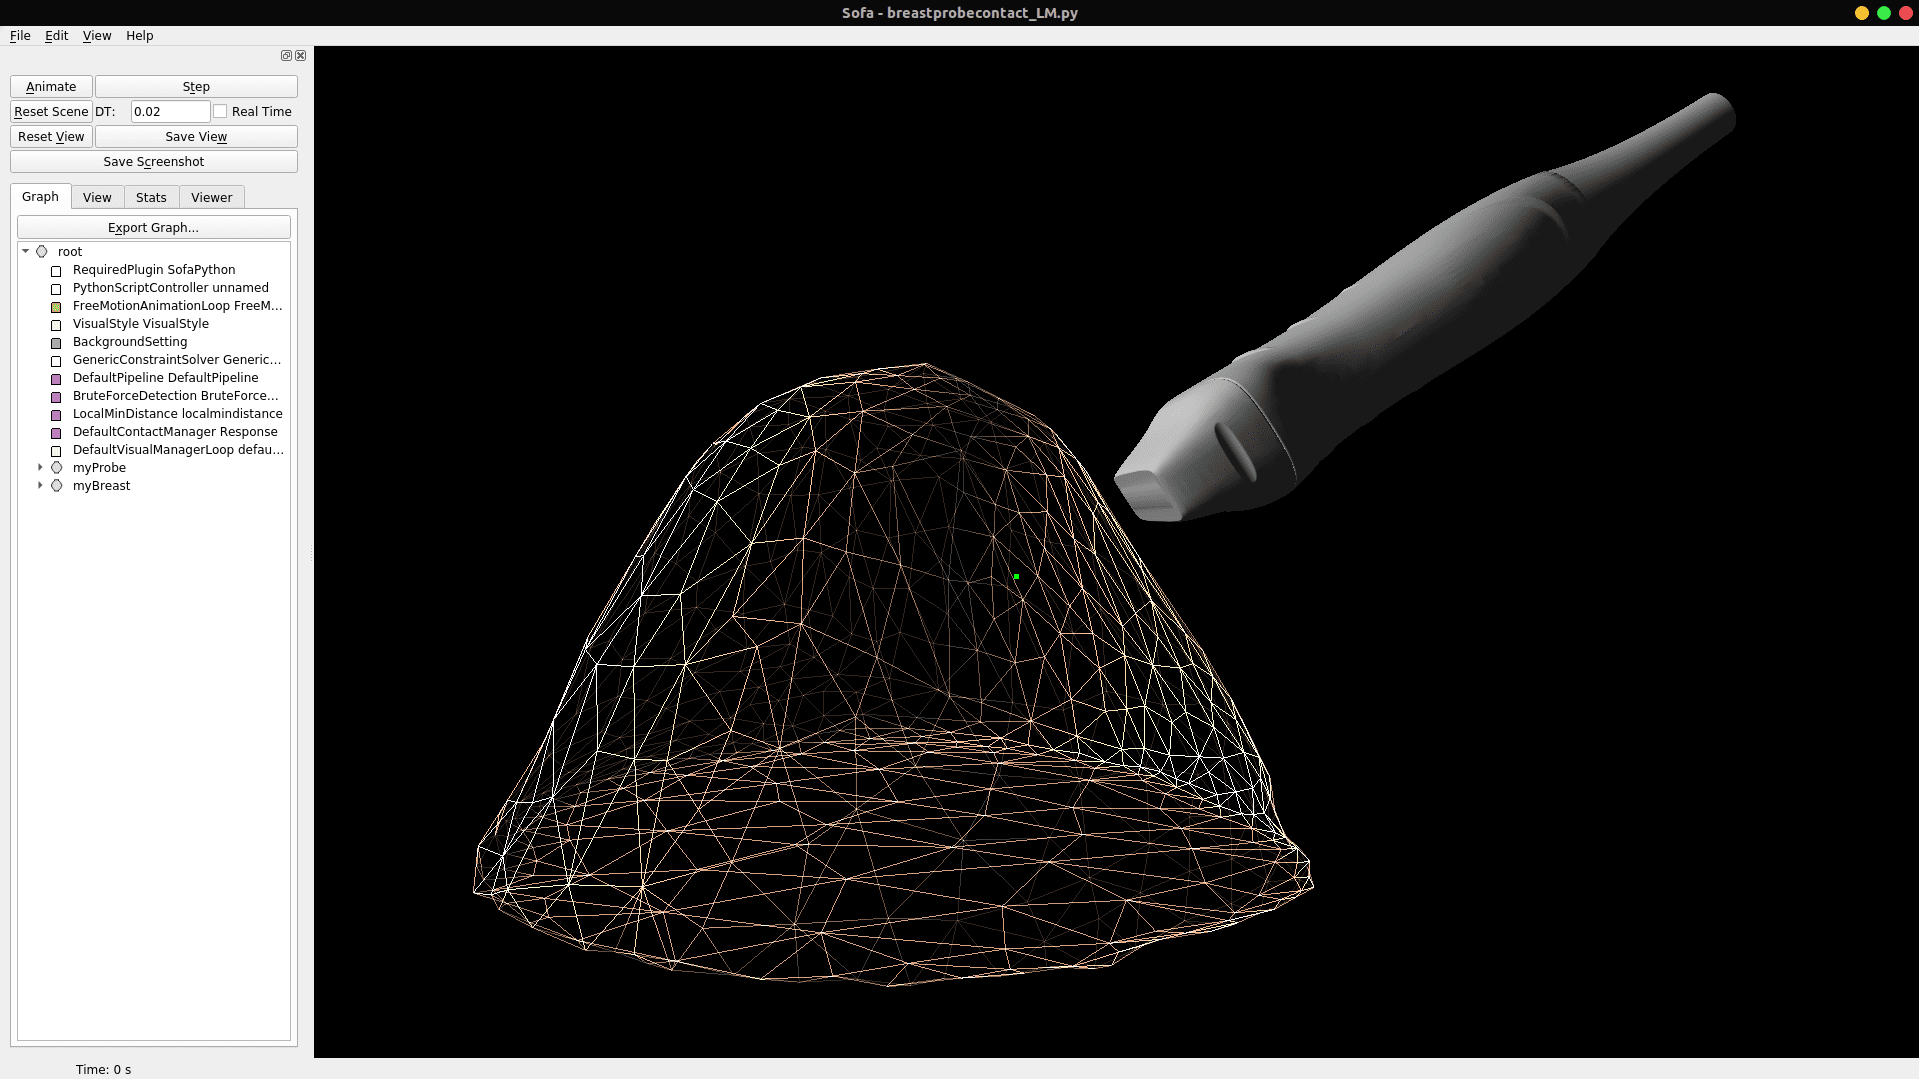
\includegraphics[width=0.49\textwidth]{images/future-work-sofa1.png}
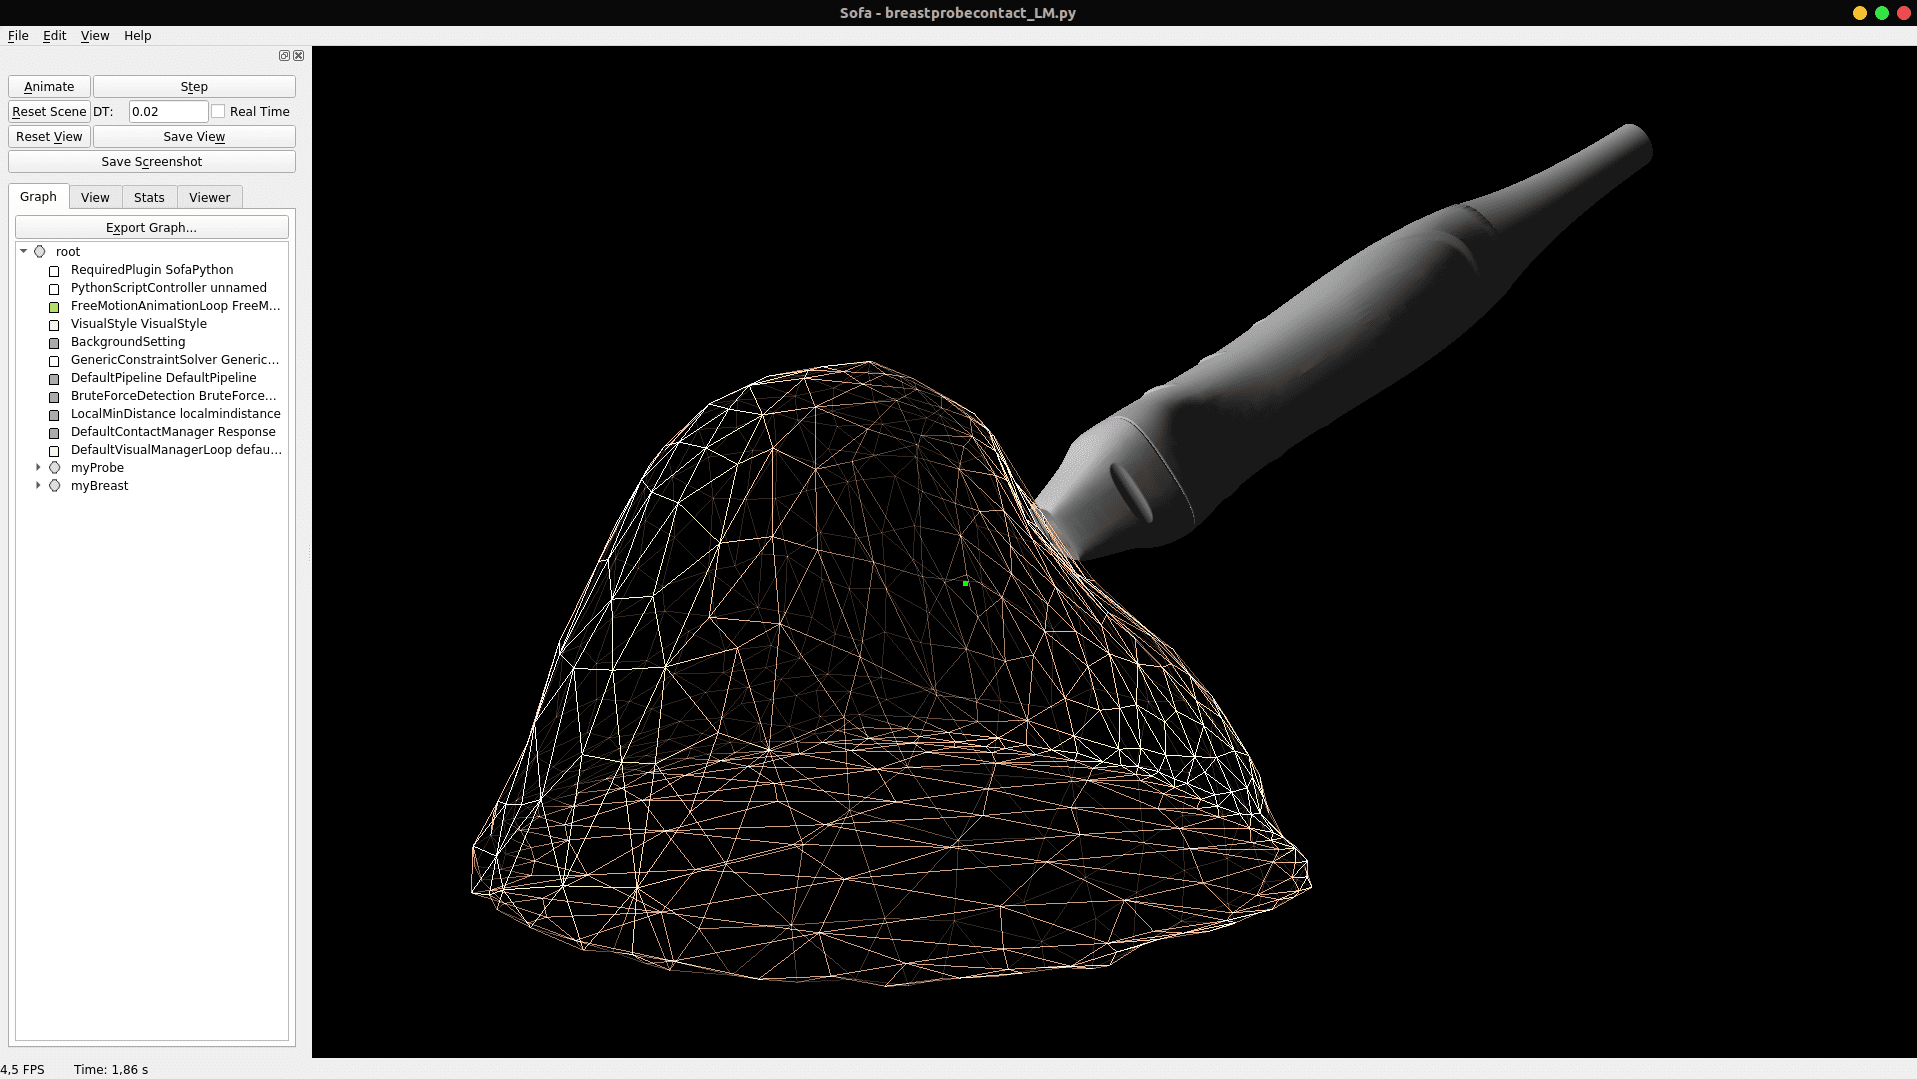
\includegraphics[width=0.49\textwidth]{images/future-work-sofa2.png}\\
\caption{Deformable tissue/organ medical simulation - Simulation of breast probing using the SOFA Framework. Screenshots from running the repository at
\url{https://gitlab.com/altairLab/probe-tissue-simulation}}
\end{figure}
\end{center}

\textbf{Advanced visualization and Haptics feedback} \\

\begin{center}
\begin{figure}[!htb]
\centering
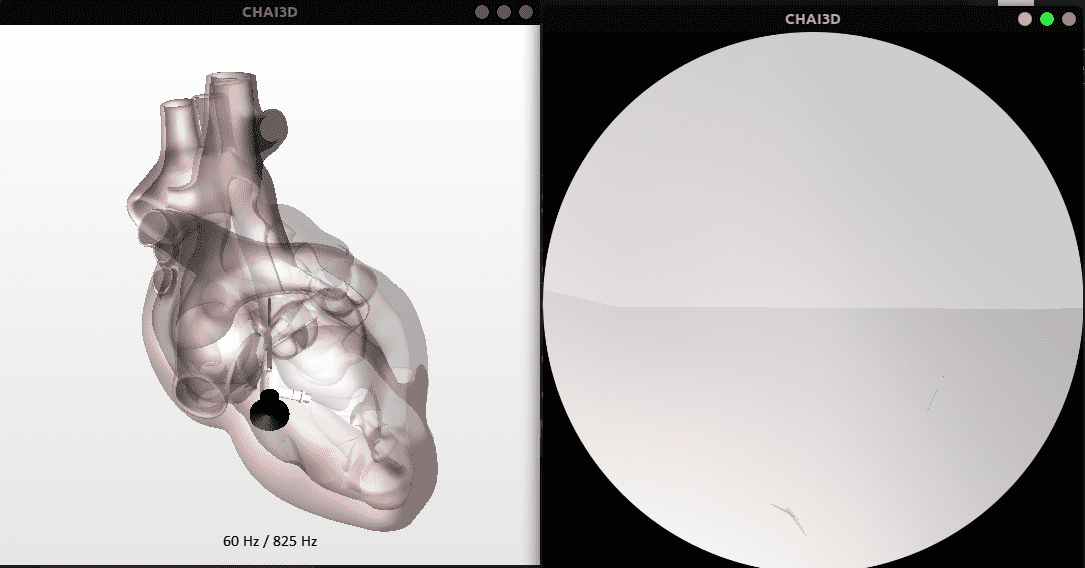
\includegraphics[width=0.7\textwidth]{images/future-work-chai3d.png}\\
\caption{Heart endoscopy medical simulation using the CHAI3D framework. Screenshots from running the repository at
\url{https://github.com/chai3d/chai3d}}
\end{figure}
\end{center}

\textbf{Applications of Machine Learning in Computer Vision and Path Planning} \\